\documentclass[12pt, a4paper, oneside]{report}
\usepackage[spanish]{babel}
\usepackage[utf8x]{inputenc}
\usepackage[T1]{fontenc}
\usepackage{newtxtext}
\usepackage{etoolbox}
\usepackage[autostyle, spanish=spanish]{csquotes}
\usepackage{amsmath,amssymb,amsfonts}
\usepackage[margin=2.5cm]{geometry}
\usepackage{setspace}
\usepackage{graphicx}

\usepackage[table]{xcolor}

\definecolor{negro}{HTML}{000000} % #000000
\definecolor{rojo}{HTML}{ff0000} % #ff0000
\definecolor{verde}{HTML}{2da44e} % #2da44e

\graphicspath{{./img/}}

\title{Dosier de prácticas de los Temas 3 y 4}
\author{José Ángel González Molina}
\date{\today}
\setlength{\parskip}{1em}
\setlength{\parindent}{1cm}
\onehalfspacing

\begin{document}
    \color{negro}
    \maketitle
    \clearpage

    \renewcommand{\chaptername}{Ejercicio}
    \renewcommand{\figurename}{Fig.}
    \chapter{Elabora un texto descriptivo}
        \begin{figure}[ht]
            \centering
            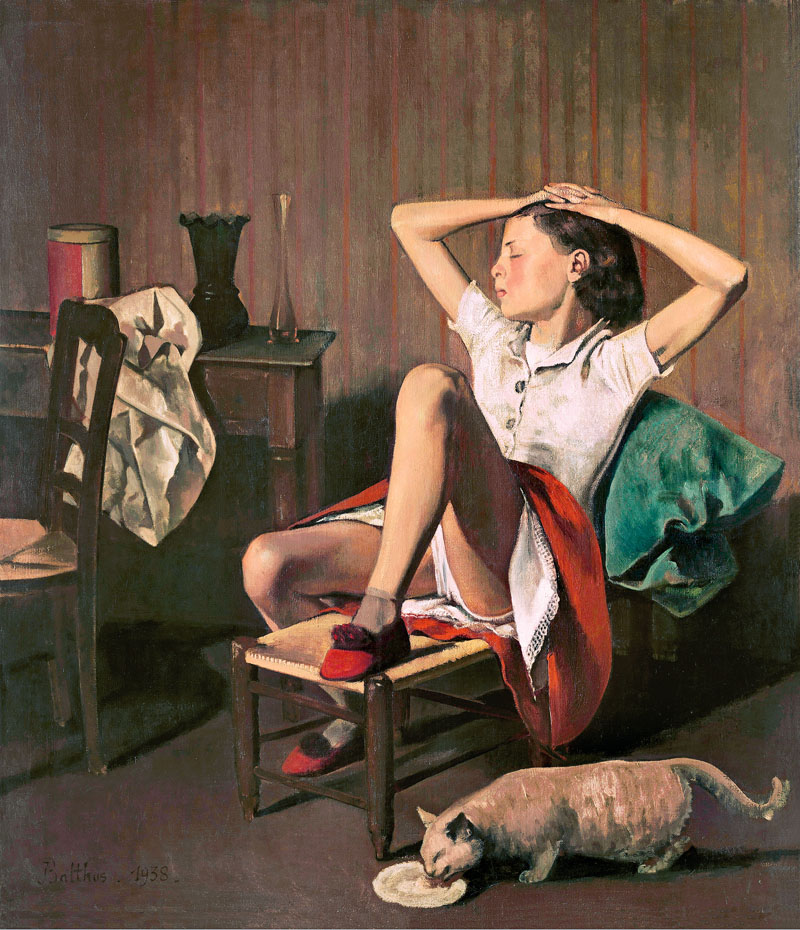
\includegraphics[scale = .75]{balthus}
            \caption{Balthus (1938). Thérèse soñando.}
        \end{figure}
        Al entrar en la habitación se encontró con Thérèse dormitando. La iluminación era tenue debido a que
        todas las lámparas se encontraban apagadas por lo que poco a poco se iban vislumbrando más detalles de
        la estancia.

        Una panorámica de la escena mostraba una toalla que se encontraba descuidadamente depositada en la
        mesa. Frente a ella, una silla mal colocada. En el centro se podía observar a la pequeña recostada en
        un cojín esmeralda, el cual recogía su espalda. Finalmente en el suelo, junto a ella, un felino níveo
        como la leche ajeno en apariencia al sopor de su compañera de juegos. Aquel día Thérèse estaba vestida
        con una camisa blanca y su habitual falda escarlata. Apoyada totalmente en el respaldo y con los
        brazos detrás de su cabeza, ojos cerrados y semblante apaciguado.

        Parecía que las tareas domésticas habían sido interrumpidas por el cansancio, o al menos eso decía el
        estado desordenado de la habitación. Pensó en despertarla, pero si no lo había hecho el ruido que
        estaba haciendo el gato con el plato, era porque el descanso era merecido.
        \clearpage
    \chapter{Elabora una introducción breve de un trabajo cuyo índice es el siguiente:}
        \section*{Índice}
        \begin{Large}
            \renewcommand{\labelenumii}{\arabic{enumi}.\arabic{enumii}}
            \begin{enumerate}
                \item Los orígenes del hombre
                \item Antes del \emph{Homo sapiens}. Los colonizadores del Viejo Mundo
                \item Los neandertales: ¿los primeros hombres modernos?
                \begin{enumerate}
                    \item Los primeros artistas
                    \item Pastores y agricultores
                \end{enumerate}
                \item Conclusiones
                \item Bibliografía
            \end{enumerate}
        \end{Large}
        \clearpage
        \section*{Introducción}

    En el presente trabajo se investigarán las poblaciones humanas en Europa en el periodo de tiempo anterior
    al apogeo del Homo sapiens. El \emph{Homo sapiens} es la especie a la que pertenecen todos los seres humanos que
    viven en la actualidad. Como se verá existieron multitud de homínidos \emph{hominina}, es decir, la
    familia de primates bípedos a la que pertenecemos y que contiene a otras especies que también poblaron
    Europa como el \emph{Homo antecessor}, el \emph{Homo heidelbergensis} y el \emph{Homo neanderthalensis}.
    Nos centraremos principalmente en los neandertales y en cómo colonizaron Europa llegando a compartir
    periodo temporal con nuestra especie.

	A lo largo de la historia de la antropología y la paleontología, ha existido una dificultad clara a la
    hora de catalogar con exactitud las especies y momentos temporales implicadas en la colonización del
    continente europeo. Una de las tesis que más aceptación tiene es la capacidad de creación de arte o
    el empleo de técnicas para seleccionar animales a convertir en ganado o semillas que cultivar. Pero
    ¿son los \emph{Homo sapiens} los primeros en conseguir estos logros? Como se expondrá en el capítulo sobre
    los neandertales, las nuevas evidencias y hallazgos nos inducen a pensar en que dichos logros fueron
    logrados con anterioridad.


\end{document}
